\documentclass[11pt,a4paper]{article}
\usepackage[margin=2cm]{geometry}
\usepackage{amsmath,amssymb,amsthm}
\usepackage{tikz}
\usepackage{enumitem}
\usepackage[hidelinks]{hyperref}
\usepackage{titlesec}
\usepackage{xcolor}

\definecolor{accent}{HTML}{1F4E79}
\titleformat{\section}{\large\bfseries\color{accent}}{\thesection.}{0.5em}{}
\titlespacing*{\section}{0pt}{1.2em}{0.4em}
\setlist{itemsep=2pt,topsep=4pt}
\setlength{\parindent}{0pt}
\setlength{\parskip}{4pt}
\hypersetup{pdftitle={Right angles on a line},pdfauthor={Krishnan}}

\newtheorem*{theorem}{Theorem}

\begin{document}

{\LARGE\bfseries\color{accent} Right angles on a line}\par
\vspace{2pt}
{\small Kind: Problem \quad Date: 12-11-2026}
\vspace{6pt}\hrule\vspace{6pt}

\section{The problem}
For some points of the form $(k,7)$, the points $A(2,3)$, $B(12,13)$ and $(k,7)$ form a
right-angled triangle. Suppose that $C$ is such a point so that $\triangle ABC$ is
right-angled at $C$. Suppose that $D$ is also such a point so that $\triangle ABD$ is
right-angled at $D$ ($D \ne C$). What is the area of $ACBD$?

\textbf{What it asks:}
\begin{enumerate}
  \item Points of the form $(k,7)$ all lie on the horizontal line $y = 7$.
  \item ``Right-angled at $C$'' means sides $CA$ and $CB$ are perpendicular.
        Find the two points $C$ and $D$ on $y=7$ where this happens.
  \item Join $A \to C \to B \to D \to A$ and find the area of this quadrilateral.
\end{enumerate}

\section{The idea in one line}
Perpendicular lines have slopes whose product is $-1$; then the diagonal $DC$ lies on $y=7$
and splits $ACBD$ into two triangles with the same base.

\section{Key parts}
\begin{enumerate}
  \item \textbf{Test one point.} $P(14,7)$: slope $AP = \tfrac{4}{12} = \tfrac13$,
        slope $PB = \tfrac{6}{-2} = -3$. Product $= -1$, so the angle at $P$ is $90^\circ$.
        (Watch the sign: from $P$ to $B$, $x$ goes from 14 down to 12.)
  \item \textbf{Find every such point.} Replace 14 by $k$ and solve.
  \item \textbf{Split the area.} $DC$ is horizontal, so each triangle's height is a
        vertical distance from the line $y = 7$.
\end{enumerate}

\section{Worked solution}
\textbf{Finding $C$ and $D$.} For the point $(k,7)$:
\[
\text{slope to } A = \frac{7-3}{k-2} = \frac{4}{k-2}, \qquad
\text{slope to } B = \frac{7-13}{k-12} = \frac{-6}{k-12}.
\]
Perpendicular:
\[
\frac{4}{k-2}\cdot\frac{-6}{k-12} = -1
\;\Rightarrow\; (k-2)(k-12) = 24
\;\Rightarrow\; k^2 - 14k = 0 \;\Rightarrow\; k(k-14) = 0
\;\Rightarrow\; k = 0 \text{ or } 14.
\]
So $C = (14,7)$ and $D = (0,7)$.

\begin{minipage}[c]{0.58\linewidth}
\textbf{Area.} Base $DC = 14$.\
Height of $\triangle DCB$: $13 - 7 = 6$.\
Height of $\triangle DCA$: $7 - 3 = 4$.
\[
\text{Area} = \tfrac12\cdot 14\cdot 6 + \tfrac12\cdot 14\cdot 4 = 42 + 28 = \boxed{70}.
\]
\end{minipage}\hfill
\begin{minipage}[c]{0.38\linewidth}
\centering
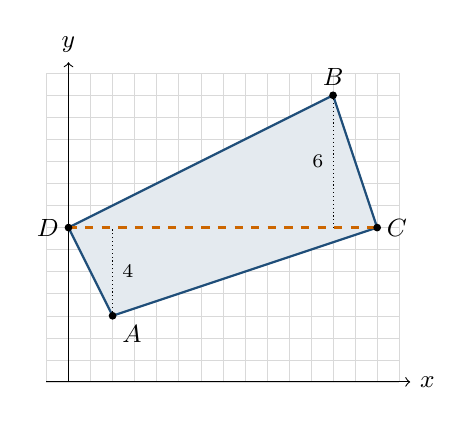
\begin{tikzpicture}[scale=0.28]
  \draw[gray!30,very thin] (-1,0) grid (15,14);
  \draw[->] (-1,0) -- (15.5,0) node[right] {\small $x$};
  \draw[->] (0,0) -- (0,14.5) node[above] {\small $y$};
  \fill[accent!12] (2,3) -- (14,7) -- (12,13) -- (0,7) -- cycle;
  \draw[accent,thick] (2,3) -- (14,7) -- (12,13) -- (0,7) -- cycle;
  \draw[orange!80!black,thick,dashed] (0,7) -- (14,7);
  \draw[densely dotted] (12,13) -- (12,7);
  \draw[densely dotted] (2,3) -- (2,7);
  \node[left] at (12,10) {\scriptsize 6};
  \node[right] at (2,5) {\scriptsize 4};
  \foreach \p/\n/\pos in {{(2,3)}/A/below right,{(14,7)}/C/right,{(12,13)}/B/above,{(0,7)}/D/left}
    { \fill \p circle (5pt); \node[\pos] at \p {\small $\n$}; }
\end{tikzpicture}
\end{minipage}

\section{Questions colleagues may ask}
\begin{enumerate}
  \item \textbf{Q. Is there a method without slopes?}
        Yes. An angle subtending a diameter is $90^\circ$ (Thales' theorem), so $C$ and $D$
        lie on the circle with diameter $AB$: centre $(7,8)$, radius$^2 = 5^2 + 5^2 = 50$.
        On $y=7$: $(k-7)^2 + 1 = 50$, so $k - 7 = \pm 7$, giving $k = 0$ or $14$.
  \item \textbf{Q. Which other points $(k,7)$ give a right-angled triangle?}
        Right angle at $A$: $k = -2$. Right angle at $B$: $k = 18$. The question only uses
        the two with the right angle at the point on $y=7$.
  \item \textbf{Q. Can we check the area another way?}
        The shoelace formula on $A(2,3), C(14,7), B(12,13), D(0,7)$ gives
        $\tfrac12\,|280 - 140| = 70$.
\end{enumerate}

\end{document}
